\begin{figure}
\centering
\newcommand{\myWidth}{0.9\textwidth}

\begin{subfigure}{\myWidth}
  \centering
  \caption{Network width $N=200$}
  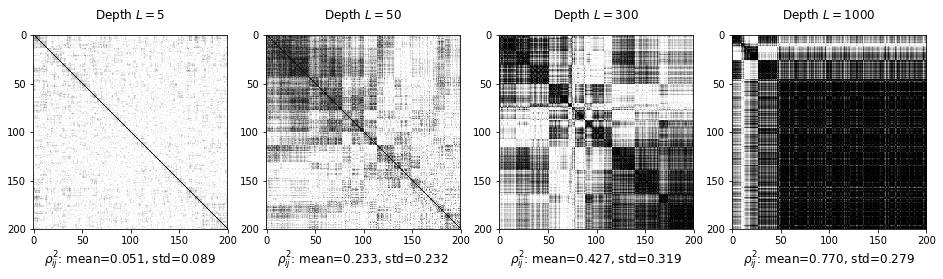
\includegraphics[width=1.0\linewidth]{mnist_FixN=200}
  \label{fig:sec4_sim3_a}
\end{subfigure}\hspace{3mm}%
\begin{subfigure}{7mm}
  \centering
  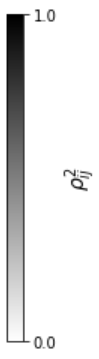
\includegraphics[width=1.0\linewidth]{colorbar}
\end{subfigure}%

\begin{subfigure}{\myWidth}
  \centering
  \caption{Network depth $L=100$}
  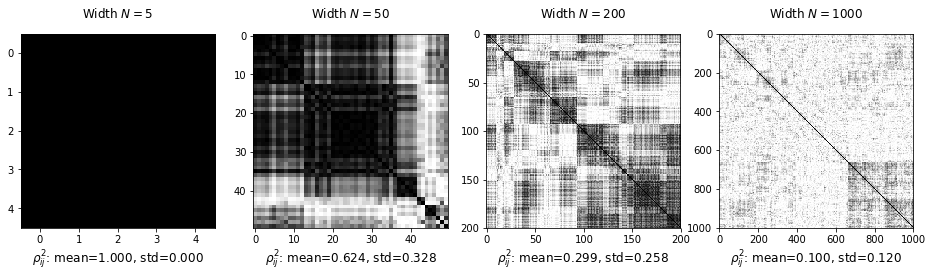
\includegraphics[width=1.0\linewidth]{mnist_FixL=100}
  \label{fig:sec4_sim3_b}
\end{subfigure}\hspace{3mm}%
\begin{subfigure}{7mm}
  \centering
  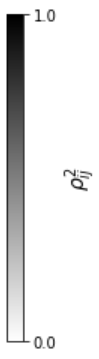
\includegraphics[width=1.0\linewidth]{colorbar}
\end{subfigure}%

\caption[The magnitudes of correlation coefficient $\rho_{ij}$ between output nodes.]{The magnitudes of correlation coefficient $\rho_{ij}$ between output nodes.
The black color means $\rho_{ij}^2=1$ while the white color indicates $\rho_{ij}^2=0$.
The top row shows that the correlation is positive related to the network depth $L$, and the bottom row presents that the correlation is negatively related to the network width $N$. Note that we rearrange the node index to cluster the correlated nodes.}
\label{fig:sec4_sim3}
\end{figure}
